\documentclass[border=4pt]{standalone}
\usepackage{adjustbox}
\usepackage{tikz}
\usetikzlibrary{positioning,arrows.meta}
\begin{document}
% Coordinates:
%   u at (1.5, 1.2)
%   x at (0, 0)
%   y at (3, 0)
\begin{adjustbox}{max width=\textwidth}
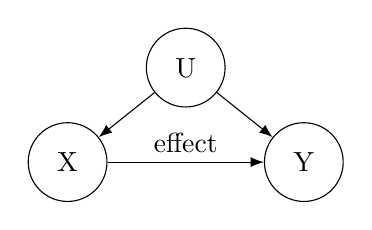
\begin{tikzpicture}[node distance=14mm and 16mm]
\node[draw, circle, minimum width=10mm, minimum height=10mm] (u) at (1.5,1.2) {U};
\node[draw, circle, minimum width=10mm, minimum height=10mm] (x) at (0,0) {X};
\node[draw, circle, minimum width=10mm, minimum height=10mm] (y) at (3,0) {Y};
\draw[-{Latex}] (u) -- (x);
\draw[-{Latex}] (u) -- (y);
\draw[-{Latex}] (x) -- node[above] {effect} (y);
\end{tikzpicture}
\end{adjustbox}
\end{document}
